\begin{frame}{2.3.6 ガウス分布に対するベイズ推論}
 \begin{itemize}
  \item 今までは最尤推定の枠組みのガウス分布パラメータ$\bm{\mu}$と$\bm{\Sigma}$の点推定量を得た
  \item 次に、事前分布を導入してベイズ主義的に扱う
  \item まずは1変数のガウス確率関数$x$について考える
        \begin{itemize}
         \item 分散が既知のとき
         \item 平均が既知のとき
         \item 平均も分散も未知のとき
        \end{itemize}
 \end{itemize}
\end{frame}

\begin{frame}{分散が既知のときの事前分布}
 \begin{itemize}
  \item \alert{分散$\sigma^2$は既知}とし、与えられた$N$個の観測値集合$\bm{x}=\{x_1,...,x_N\}$から、平均$\mu$を推定する
  \item $\mu$が与えられたときに観測データが生じる確率である尤度関数は$\mu$の関数と見なせて、
        \begin{eqnarray*}
         p(\bm{X}|\mu) &= &\prod_{n=1}^{N}p(x_n|\mu) \\
         &=& \frac{1}{(2\pi\sigma^2)^{N/2}}\exp\left\{-\frac{1}{2\sigma^2}\sum_{n=1}^{N}(x_n-\mu)^2\right\}
        \end{eqnarray*}
  % \item ただし、尤度関数は$\mu$上の確率分布ではなく、正規化もされていない
  \item 尤度関数を見ると、$\mu$についての二次形式の指数の形を取っている
  \item 前事分布$p(\mu)$にガウス分布を選べば、この尤度関数の共役事前分布となる
 \end{itemize}
\end{frame}

\begin{frame}{事後分布}
 \begin{itemize}
  \item 事前分布を次のようにする
        \begin{equation}
         p(\mu) = \mathcal{N}(\mu|\mu_0,\sigma_0^2)
        \end{equation}
  \item すると事後分布は
        \begin{eqnarray}
         p(\mu|\bm{X})&=&\frac{p(\bm{X}|\mu)p(\mu)}{p(\bm{X})} \nonumber \\
         &\propto &p(\bm{X}|\mu)p(\mu)
        \end{eqnarray}
        となる
 \end{itemize}
\end{frame}

\begin{frame}{事後分布の平均と分散}
 \begin{itemize}
  \item 事後分布の指数部分は、
        \begin{eqnarray}
         & &\exp\left\{-\frac{1}{2\sigma_0^2}(\mu-\mu_0)^2\right\} \exp\left\{-\frac{1}{2\sigma^2}\sum_{n=1}^{N}(\mu-x_n)^2\right\} \nonumber \\
         &= & \exp\left\{-\frac{1}{2}\left(\frac{1}{\sigma_0^2}+\frac{N}{\sigma^2}\right)\mu^2 +\left(\frac{\mu_0}{\sigma_0^2}+\frac{1}{\sigma^2}\sum_{n=1}^{N}x_n\right)\mu +C_0 \right\} \nonumber
        \end{eqnarray}
  \item 平方完成と正規化によって平均$\mu_N$,分布$\sigma_N^2$のガウス分布の形にすることができる。ただし、
        \begin{eqnarray}
         \mu_N& = & \frac{\sigma^2}{N\sigma_0^2+\sigma^2}\mu_0 + \frac{N\sigma_0^2}{N\sigma_0^2+\sigma^2}\mu_{ML}\label{223654_18Nov14}\\
         \frac{1}{\sigma_N^2}&= & \frac{1}{\sigma_0^2} + \frac{N}{\sigma^2}\label{181817_24Nov14}\\
         \mu_{ML}&= & \frac{1}{N}\sum_{n=1}^{N}x_n
        \end{eqnarray}
 \end{itemize}
\end{frame}

\begin{frame}{平均と分散の性質}
 \begin{eqnarray}
  \mu_N& = & \frac{\sigma^2}{N\sigma_0^2+\sigma^2}\mu_0 + \frac{N\sigma_0^2}{N\sigma_0^2+\sigma^2}\mu_{ML}\label{181902_24Nov14}\\
  \frac{1}{\sigma_N^2}&= & \frac{1}{\sigma_0^2} + \frac{N}{\sigma^2}
 \end{eqnarray}
 \begin{itemize}
  \item $N\rightarrow0$なら、予想通り式(\ref{181902_24Nov14})は事前分布の平均
  \item $N\rightarrow\infty$なら、事後分布の最尤推定解となる
  \item 事後分布の精度は事前分布の精度に各観測データ点からのデータ精度への影響分を加えたものになる
        \begin{itemize}
         \item データ点が増えるにつれ、精度が確実に増加する
        \end{itemize}
  % \item $N\rightarrow0$なら、事前分布の分散に一致
  % \item $N\rightarrow\infty$なら、分散は最尤推定解に一致
 \end{itemize}
\end{frame}

\begin{frame}{事後分布のもう一つの見方}
 \begin{itemize}
  \item ガウス分布の逐次推定では、$N$個のデータ点を観測した後の平均は$N$番目のデータ点$x_N$の影響と$N-1$個のデータ点を観測した後の平均とでも表現できた
  \item このことをガウス分布の平均の推論の場合について示す
        \begin{equation}
         p(\mu|\bm{X}) \propto
          \! \! \! \! \! \! \! \! \! \! \! \! \! \! \! \! \!\underbrace{\left[p(\mu)\prod_{n=1}^{N-1}p(x_n|\mu)\right]}_{\mbox{{\scriptsize $N-1$個のデータ点を観測した後の事後分布}}}
          \! \! \! \! \! \! \! \! \! \! \! \! \! \! \! \! \! p(x_N|\mu)
        \end{equation}
  % \item カギカッコ内の項は正規化係数を除いて、$N-1$個のデータ点を観測した後の事後分布にちょうど一致する
  \item この項を事前分布とし、データ点$x_N$についての尤度関数をベイズの定理によって結合すれば、この式全体は$N$個のデータ点を観測した後の事後分布とみなせる
 \end{itemize}
\end{frame}

\begin{frame}{分散が既知の場合:$N$が増えたときの事後分布の変化}
 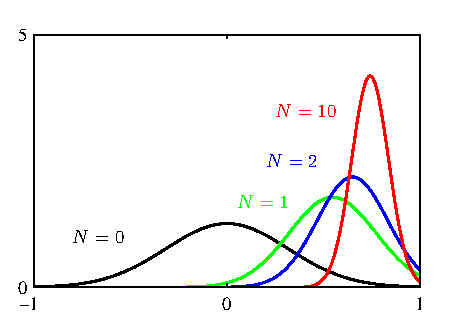
\includegraphics[width=\textwidth]{./figure/Figure2.12.eps}
\end{frame}

\begin{frame}{平均が既知の場合}
 \begin{itemize}
  % \item \alert{平均が既知}の場合、事前分布に共役な分布を選ぶと計算が単純化
  \item 簡単のため、精度$\lambda\equiv 1/\sigma^2$で操作する
  \item 尤度は次のようになる
        \begin{eqnarray}
         p(\bm{X}|\lambda) &=& \prod_{n=1}^{N}\mathcal{N}(x_n|\mu,\lambda^{-1}) \nonumber \\
         &=& \lambda^{N/2}\exp\left\{-\frac{\lambda}{2}\sum_{n=1}^{N}(x_n-\mu)^2\right\}\label{114403_19Nov14}
        \end{eqnarray}
  \item この式から、精度の共役事前分布は、$\lambda$のベキ乗と、$\lambda$の線形関数の指数の積に比例させる
        \begin{itemize}
         \item \alert{ガンマ分布}
        \end{itemize}
 \end{itemize}
\end{frame}


\begin{frame}{ガンマ分布}
 \begin{itemize}
  \item ガンマ分布の定義
        \begin{equation}
         {\rm Gam}(\lambda|a,b) = \frac{1}{\Gamma(a)}b^a\lambda^{a-1}\exp(-b\lambda)\label{113739_19Nov14}
        \end{equation}
  \item ここで、$\Gamma(a)$は式(\ref{113739_19Nov14})が正しく正規化されることを保証
  \item ガンマ分布の平均と分散は
        \begin{eqnarray}
         \mathbb{E}[\lambda] &=& \frac{a}{b}\\
         {\rm var}[\lambda]& =& \frac{a}{b^2}
        \end{eqnarray}
 \end{itemize}
 \begin{tabular}[tb]{ccc}
  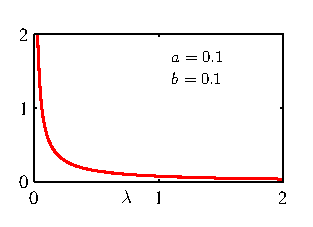
\includegraphics[width=0.33\textwidth]{./figure/Figure2.13a.eps}
  &
  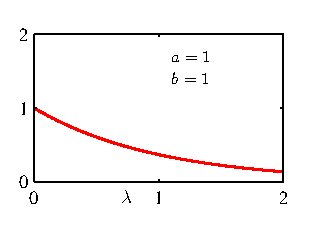
\includegraphics[width=0.33\textwidth]{./figure/Figure2.13b.eps}
  &
  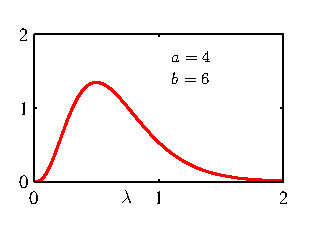
\includegraphics[width=0.33\textwidth]{./figure/Figure2.13c.eps}
 \end{tabular}
\end{frame}

\begin{frame}{事後分布}
 \begin{itemize}
  \item 事前分布${\rm Gam}(\lambda|a_0,b_0)$に尤度関数(\ref{114403_19Nov14})をかけると、事後分布
        \begin{equation}
         p(\lambda|\bm{X}) \propto \lambda^{a_0-1}\lambda^{N/2}\exp\left\{-b_0\lambda-\frac{\lambda}{2}\sum_{n=1}^{N}(x_n-\mu)^2\right\}\label{114734_19Nov14}
        \end{equation}
        が得られる
        \begin{itemize}
         \item 正しい係数は後から簡単に求められるため、事前分布や尤度関数で正規化係数を維持更新する必要はない
        \end{itemize}
  \item これはパラメータを次のように設定したときの、ガンマ分布${\rm Gam}(\lambda|a_N,b_N)$であることが分かる
        \begin{eqnarray}
         a_N&=& a_0 + \frac{N}{2}\\
         b_N% &= & b_0+\frac{1}{2}\sum_{n=1}^{N}(\bm{x}_n-\mu)^2\\
         &= & b_0+\frac{N}{2}\sigma^2_{ML}
        \end{eqnarray}
 \end{itemize}
\end{frame}

\begin{frame}{事前分布のパラメータの解釈}
 \begin{eqnarray*}
  a_N&=& a_0 + \frac{N}{2}\\
  b_N% &= & b_0+\frac{1}{2}\sum_{n=1}^{N}(\bm{x}_n-\mu)^2\\
  &= & b_0+\frac{N}{2}\sigma^2_{ML}
 \end{eqnarray*}
 \begin{itemize}
  \item $a_0$は、$2a_0$個の「有効な」観測値が事前にあると解釈できる
  \item $b_0$は、その分散が$b_0/a_0$であるような、$2a_0$個の「有効な」観測値が事前にあると解釈できる
 \end{itemize}
\end{frame}

% \begin{frame}{パラメータの性質}
%  \begin{itemize}
%   \item 式(\ref{114734_19Nov14})では、事前分布や尤度関数で正規化係数を維持更新する必要はない
%         \begin{itemize}
%          \item 必要に応じて、正規化されたガンマ分布(\ref{113739_19Nov14})を用いて正しい係数を求めることができるため
          %         \end{itemize}
          %   \item 式(\ref{115004_19Nov14})より、$N$個のデータ点を観測すると、係数$a$を$N/2$だけ増やす効果がある
          %         \begin{itemize}
          %          \item 事前分布のパラメータ$a_0$は、$2a_0$個の「有効な」観測値が事前にあると解釈できる
                    %         \end{itemize}
                    %   \item 式(\ref{115046_19Nov14})より、$N$個のデータ点は$N\sigma_{ML}^2/2$だけ、パラメータ$b$に影響を及ぼす
                    %         \begin{itemize}
                    %          \item 事前分布のパラメータ$b_0$は、その分布が$b_0/a_0$であるような、$2a_0$個の「有効な」観測値が事前にあると解釈できる
                              %         \end{itemize}
   %  \end{itemize}
  % \end{frame}


  \begin{frame}{逆ガンマ分布}
   \begin{itemize}
    \item 今までは精度について考えて、ガンマ分布を導入した
    \item 一方、分散そのものについて考えることもできる
          \begin{itemize}
           \item \alert{逆ガンマ分布}
                 \begin{itemize}
                  \item ここでは触れない
                 \end{itemize}
          \end{itemize}
   \end{itemize}
  \end{frame}

  \begin{frame}{平均と分散が未知の場合}
   \begin{itemize}
    \item \alert{平均と分散が未知}の場合には、共役事前分布を求めるために尤度関数の$\mu$と$\lambda$への依存関係について考える
          \begin{eqnarray}
           p(\bm{X}|\mu,\lambda) &=& \prod_{n=1}^{N}\left(\frac{\lambda}{2\pi}\right)^{1/2}\exp\left\{-\frac{\lambda}{2}(x_n-\mu)^2\right\} \nonumber \\
           &\propto & \! \! \left[\lambda^{1/2}\exp\left(-\frac{\lambda\mu^2}{2}\right)\right]^{N}
            \! \! \!\exp\left\{\lambda\mu\sum_{n=1}^{N}x_n-\frac{\lambda}{2}\sum_{n=1}^{N}x_n^2\right\} \nonumber \\
           & &
          \end{eqnarray}
   \end{itemize}
  \end{frame}

  \begin{frame}{事後分布}
   \begin{itemize}
    \item ここでは、尤度関数と同じ$\mu$と$\lambda$への関数依存性を備えた事前分布$p(\mu,\lambda)$を求めたいので、分布は次の形式になる
          \begin{eqnarray}
           p(\mu,\lambda) &\propto& \left[\lambda^{1/2}\exp\left(-\frac{\lambda\mu^2}{2}\right)\right]^\beta \exp\left\{c\lambda\mu-d\lambda\right\} \nonumber \\
           &= & \underbrace{\exp\left\{-\frac{\beta\lambda}{2}(\mu-c\beta)^2\right\}\lambda^{\beta/2}}_{{\small \mbox{$p(\mu|\lambda)$:ガウス分布}}}
            \underbrace{\exp\left\{-\left(d-\frac{c^2}{2\beta}\right)\lambda\right\}}_{{\small \mbox{$p(\lambda)$:ガンマ分布}}} \nonumber \\
           & &
          \end{eqnarray}
    % \item 常に$p(\mu,\lambda)=p(\mu|\lambda)p(\lambda)$と書けるので、$p(\mu|\lambda)$と$p(\lambda)$に対応する部分を見出せばよい
    % \item $p(\mu|\lambda)$は精度が$\lambda$の線形関数であるガウス分布であり、$p(\lambda)$はガンマ分布であることがわかる
    \item よって、定数$\mu_0=c/\beta, a=(1+\beta)/2,$および$b=d-c^2/2\beta$を新たに定義すると、正規化した事前分布は次の形を取る
          \begin{equation}
           p(\mu,\lambda)=\mathcal{N}(\mu|\mu_0, (\beta\lambda)^{-1}){\rm Gam}(\lambda|a,b)
          \end{equation}
    \item この分布を\alert{正規-ガンマ分布}や\alert{ガウス-ガンマ分布}と呼ぶ
   \end{itemize}
  \end{frame}

  \begin{frame}{正規-ガンマ分布の特徴}
   \begin{equation*}
    p(\mu,\lambda)=\mathcal{N}(\mu|\mu_0, (\beta\lambda)^{-1}){\rm Gam}(\lambda|a,b)
   \end{equation*}
   \begin{itemize}
    \item この分布は、独立な$\mu$上のガウス事前分布と$\lambda$上のガンマ事前分布の単純な積ではない
          \begin{itemize}
           \item $\mu$の分布の精度は$\lambda$の線形関数になっているため
          \end{itemize}
    \item たとえ$\mu$と$\lambda$が独立な事前分布を選んでも、事後分布では$\mu$の分布の精度と$\lambda$との間に関連が生じる
   \end{itemize}
  \end{frame}

  \begin{frame}{多次元変数の場合}
   \begin{itemize}
    \item これまで1次元変数の場合を考えたが、次に$D$次元変数の多変量ガウス分布の場合を考える
          \begin{itemize}
           \item 分散が既知のとき
           \item 平均が既知のとき
           \item 平均も分散も未知のとき
          \end{itemize}
    \item \alert{分散を既知}とすれば、平均$\bm{\mu}$の共役事前分布は、またガウス分布になる
          \begin{eqnarray*}
           p(\bm{X}|\mu) &=& \prod_{n=1}^{N}p(x_n|\mu)\\
           & \propto&\frac{1}{|\bm{\Sigma}|^{N/2}}\exp\left\{\sum_{n=1}^{N}-\frac{1}{2}(\bm{x}_n-\bm{\mu})^{\mathrm{T}}\bm{\Sigma}^{-1}(\bm{x}_n-\bm{\mu})\right\}
          \end{eqnarray*}
   \end{itemize}
  \end{frame}

  \begin{frame}{平均が既知の場合}
   \begin{itemize}
    \item \alert{平均が既知}で、精度行列$\bm{\Lambda}$が未知なら、共役事前分布は次式のウィシャート分布となる
          \begin{equation}
           \bm{W}(\bm{\Lambda}|\bm{W},\nu) = B|\bm{\Lambda}|^{(\nu-D-1)/2}\exp\left(-\frac{1}{2}Tr(\bm{W}^{-1}\bm{\Lambda})\right)
          \end{equation}
          % \begin{itemize}
    %  \item $\nu$は分布の自由度パラメータ
    %  \item $\bm{W}$は$D \times D$の尺度行列
    %  \item $Tr($・$)$はトレース
    %  \item $B$は次式
            % \end{itemize}
          \begin{equation}
           B(\bm{W},\nu) = |\bm{W}|^{-\nu/2}\left(2^{\nu D/2}\pi^{D(D-1)/4}\prod_{i=1}^D\Gamma\left(\frac{\nu+1-i}{2}\right)\right)^{-1}
          \end{equation}
    \item ここでも、精度行列上ではなく、共分散行列上の共役事前分布を定義できる
          \begin{itemize}
           \item 逆ウィシャート分布(ここでは触れない)
          \end{itemize}
   \end{itemize}
  \end{frame}

  \begin{frame}{平均と精度の両方が未知の場合}
   \begin{itemize}
    \item \alert{平均と精度の両方が未知}なら、1変数の場合と同様に考えることで次の共役事前分布が得られる
          \begin{equation}
           p(\bm{\mu},\bm{\Lambda}|\bm{\mu}_0,\beta,\bm{W},\nu) = \mathcal{N}(\bm{\mu}|\bm{\mu}_0,(\beta\bm{\Lambda})^{-1})\bm{W}(\lambda|\bm{W},\nu)
          \end{equation}
    \item \alert{正規-ウィシャート分布}または\alert{ガウス-ウィシャート分布}と呼ぶ
   \end{itemize}
  \end{frame}
